\chapter{Laboratorium I}\label{ch:lab-1}

\section{Wybrany sprzęt}\label{sec:lab1-hw}

Oficjalny moduł Fundacji Raspberry Pi -- \emph{Sense HAT} -- zawiera żyroskop, akcelerometr, magnetometr, barometr,
termometr, higrometr, czujnik oświetlenia, joystick, oraz~matrycę $8\,\times\,8$ pikseli RGB\thinspace\cite{sensedoc}.

Część dostępnej funkcjonalności pokrywa~się z~pozostałymi dostępnymi modułami, w~związku z~czym do~tego~laboratorium
wykorzystana~została funkcjonalność \emph{Inertial Measurement Unit} -- żyroskop, akcelerometr, magnetometr, a~także
matryca pikseli w~celu symulacji działania kompasu.

Z~powodu dużych zakłóceń magnetycznych spowodowanych obecnością metalowych elementów w~większości pomieszczeń uczelni,
utworzony kompas nie~będzie bardzo dokładny, jednak dostatecznie pokazuje działanie podobnych urządzeń np.\
w~telefonach czy~technologiach \emph{Full Body Tracking} popularyzowanych w~kręgach fanów wirtualnej rzeczywistości.
Rozwiązania~te poza~zdecydowanie bardziej wyspecjalizowanym doborze elementów sprzętowych i~bardziej zaawansowanym
oprogramowaniu kompensującym wpływ czynników zewnętrznych opierają~się fundamentalnie na~tej~samej zasadzie działania.

W~celu redukcji niedokładności instrukcja zawiera zadanie kalibracyjne, jego~wynik zależy jednak od~warunków środowiska
i~dokładności wykonania, więc~jest~jedynie krokiem referencyjnym pokazującym istnienie podobnego procesu po~stronie
producenta zintegrowanych urządzeń.

\section{Dodatkowe oprogramowanie}\label{sec:lab1-sw}

W tym laboratorium wykorzystana jest oficjalna biblioteka \emph{sense\_hat}\thinspace\cite{senselib}.
Jest to najprostszy sposób wykorzystania możliwości sensorów modułu \emph{Sense HAT}, więc stanowi łagodne wprowadzenie
do dalszych zadań w środowisku marimo.
Biblioteka udostępnia klasę \emph{SenseHat} zawierającą funkcje pomagające w wykorzystaniu czujników oraz matrycy.

\section{Rozwiązanie}\label{sec:lab1-sol}

\begin{figure}[H]
  \centering
  \includegraphics[width=0.8\linewidth]{media/sense_hat_lab}
  \caption{Fragment instrukcji \emph{Sense HAT}}
  \label{fig:sensehatlab}
\end{figure}

Na rysunku~\ref{fig:sensehat} zaprezentowany jest wynik uruchomienia rozwiązanego laboratorium.
Podobnie do~standardowego kompasu kierunki północy i~południa są~reprezentowane w~kolorach czerwonym i~białym.

\begin{figure}[H]
  \centering
  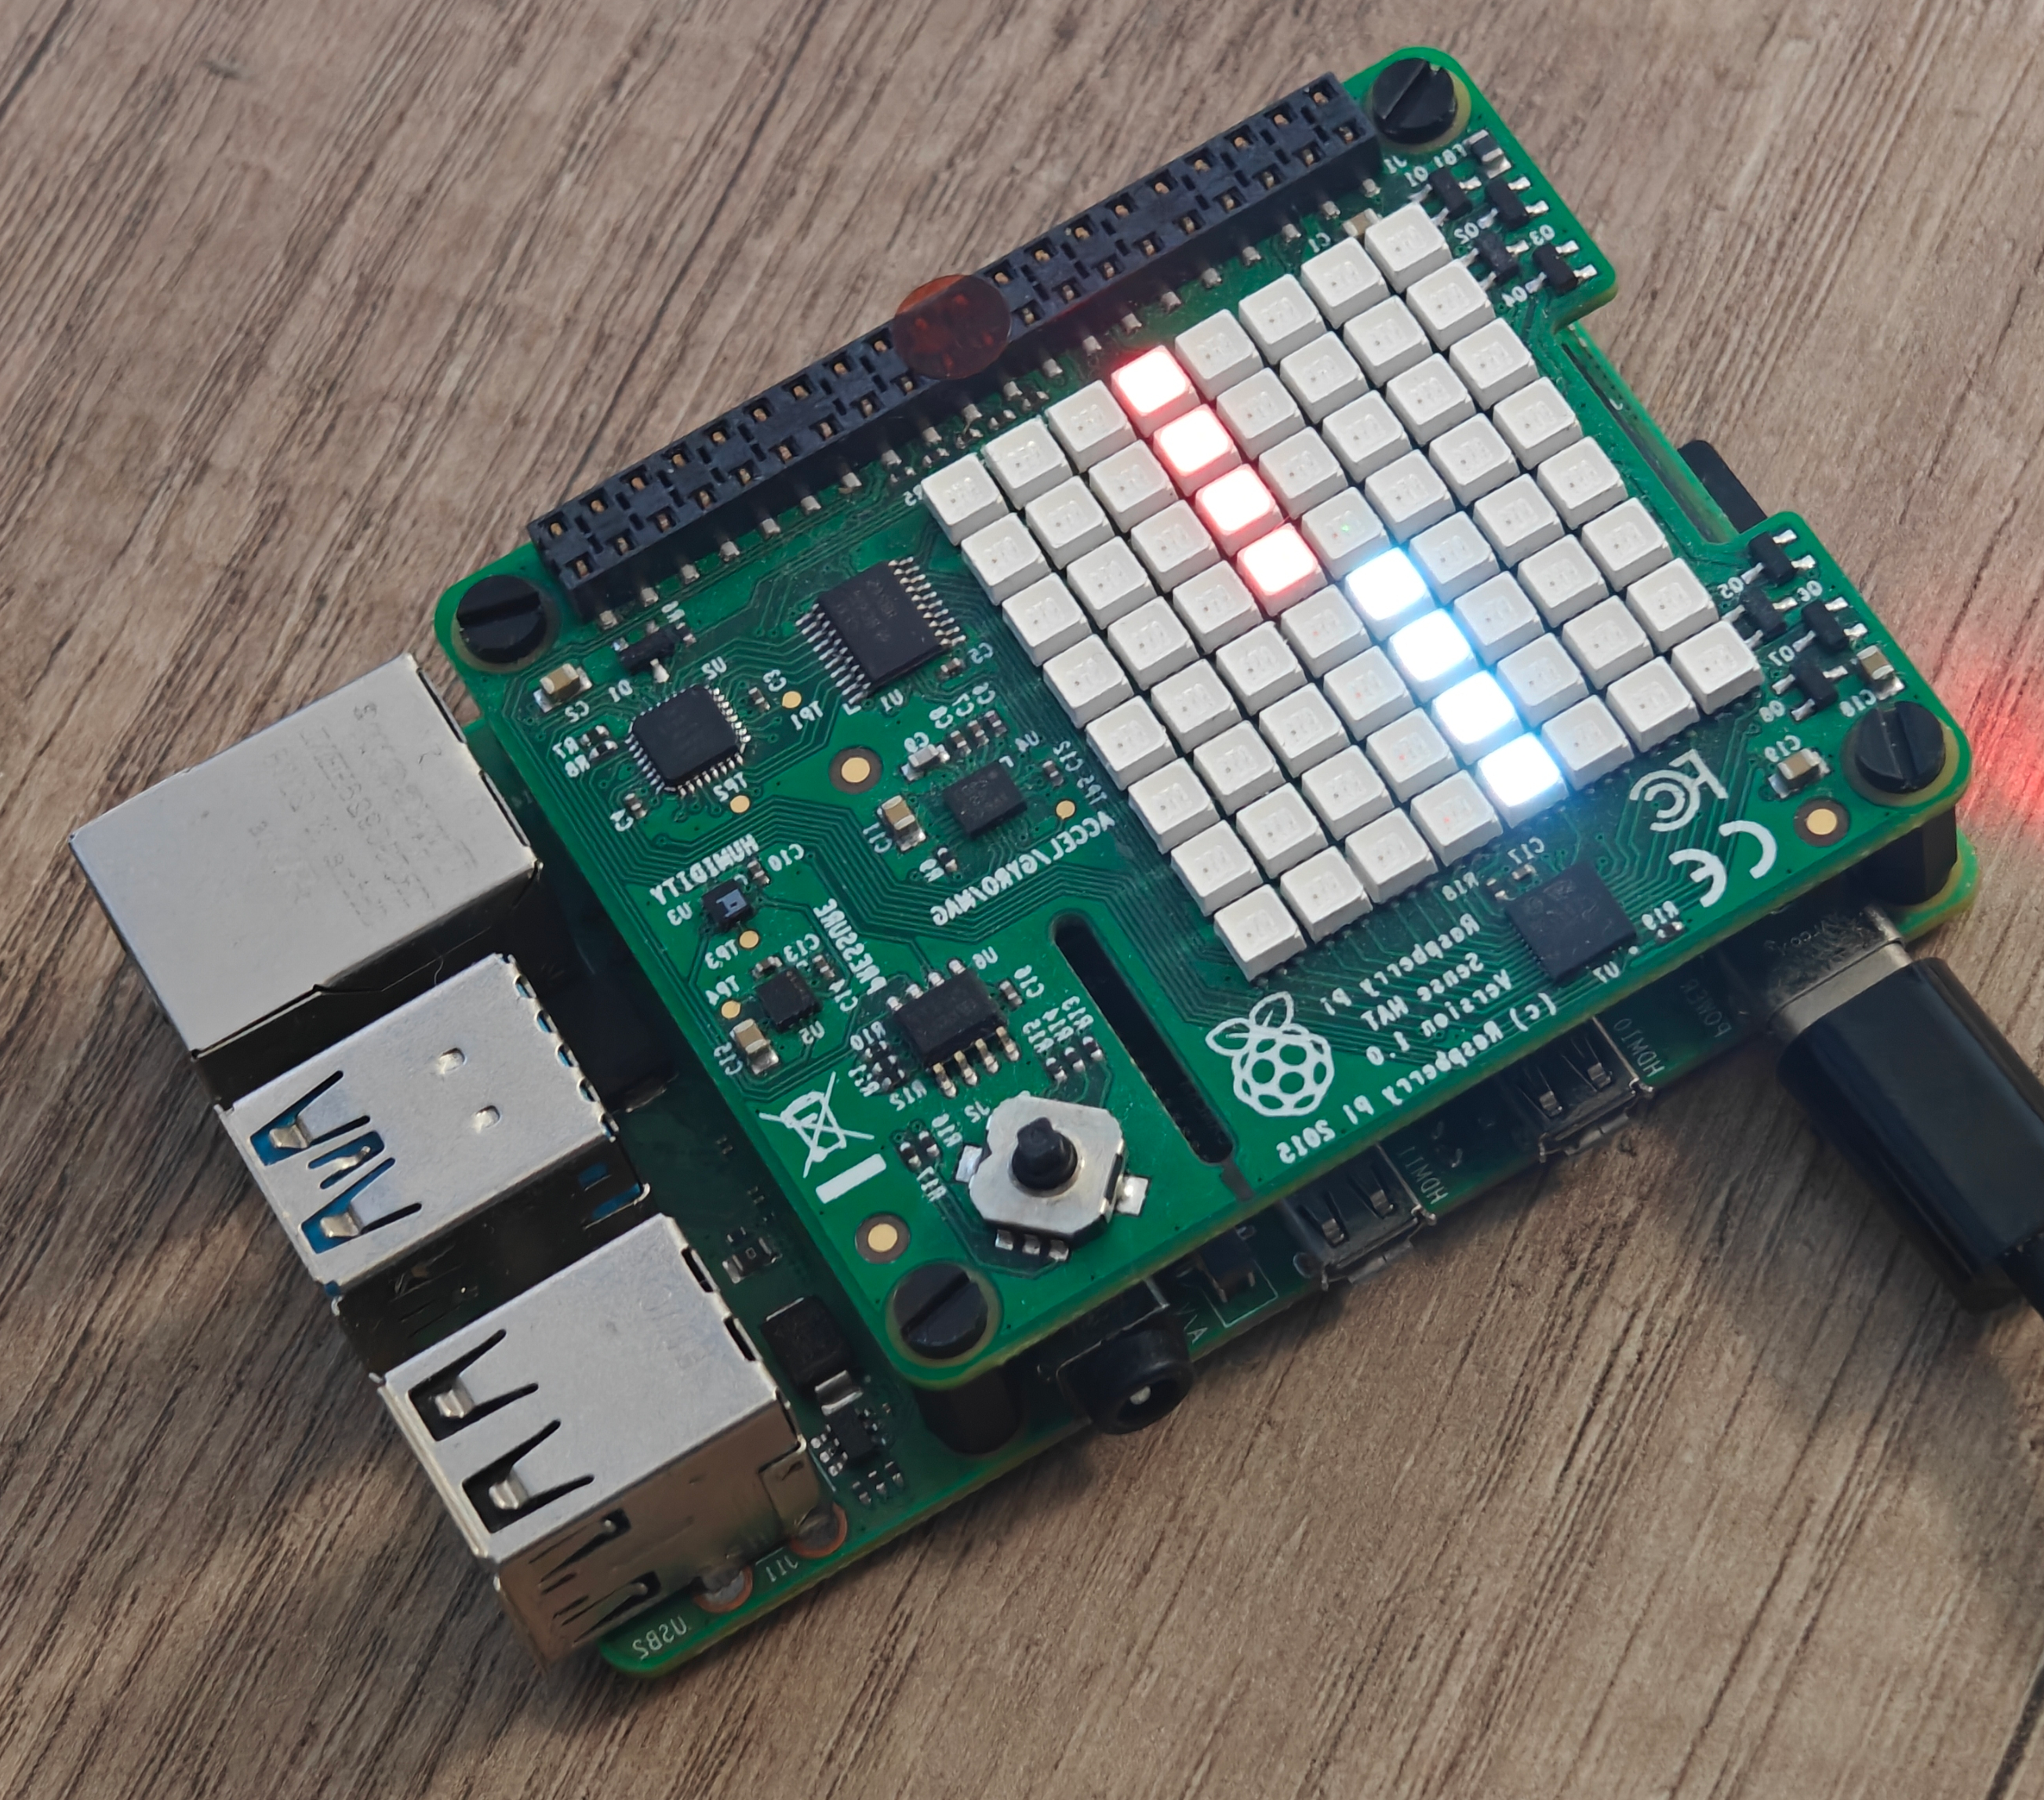
\includegraphics[width=0.6\linewidth]{media/sense_hat}
  \caption{Moduł \emph{Sense HAT} z uruchomionym programem}
  \label{fig:sensehat}
\end{figure}
